\documentclass{article}
\usepackage[utf8]{inputenc}

%\usepackage[md]{titlesec}
\usepackage{graphicx}

\setcounter{tocdepth}{1}

\renewcommand{\thesubsection}{\alph{subsection}}
%\renewcommand{\thesubsubsection}{\arabic{\subsubsection}}



\date{September 16, 2016}


\title{\textbf{Assignment 5}\\ VLSM and more on Dynamic Routing (OSPF)}
\author{s316620}
\date{September 23, 2016}

\begin{document}



\maketitle

\newpage

\tableofcontents

\newpage
\part{Introduction}

This assignment looks into the topics like subneting, VLSM and OSPF. Subnetting is dividing the Ip address into the host and network portion. Variable Length  Subnet Mask (VLSM) is a way to make subnetting more efficient. It is like subneting the subnet, it has the block size with only the amount of hosts it need and minimizes wasting of IP addresses.
OSPF (Open Shortest Path First) is a link state routing protocol based on the Dijkstra's algorithm. \cite{textbook} 

\part{Materials and Methods}

The network topology in used in this assignment is provided in the assignment paper, and the practical parts are done in the virtual machine set up in the previous assignments.

\section{VLSM (Variable Length Subnet Masking)\\ exersice 1}
Considering the network in Figure \ref{fig:network-one} we will assign each subnet a range of IP addresses. 

\begin{figure}[!h]
    \centering
    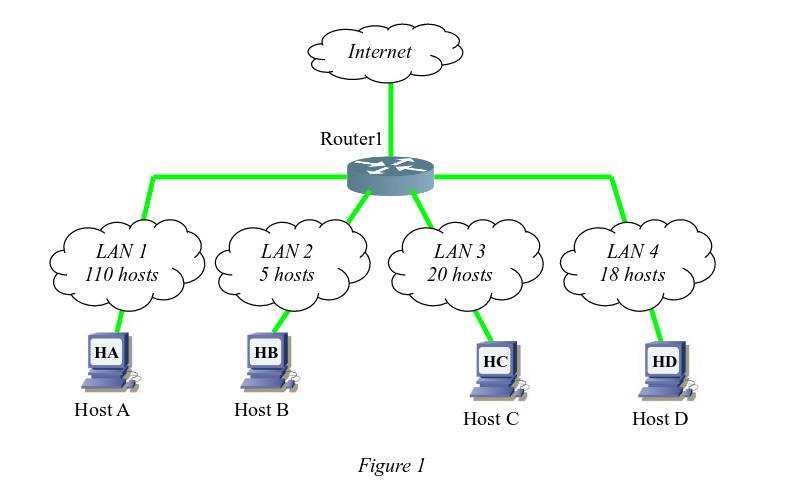
\includegraphics[scale=0.3]{5-network-one}
    \caption{Network topology from Assignment 5.}
    \label{fig:network-one}
\end{figure}

\subsection{} As there are 111 hosts on LAN1, i.e. 110 hosts specified plus a host address for the router, the IP address block allocated for LAN1 is 126. The subnet mask will be 255.255.255.128 (/25). It will be in the range 10.0.1.1 - 10.0.1.126, assigning the third IP address to Host A it will have the IP 10.0.1.3/25. 

\subsection{} The IP address and the subnet mask for LAN3 and LAN4 are 10.0.1.128/27 and 10.0.1.160/27.
If Host C is assigned the first available address in the address range of LAN3 it will have the address 10.0.1.129 and If we assign the last available address for Host D in its block it will have the address 10.0.1.190.

\subsection{} Now assigning the third available block sufficiently large enough to accommodate LAN2, it will have the network address 10.0.1.192/29. Assigning Host B the second last address in the block it will have the address 10.0.1.197. 

\subsection{} 
There are 53 address that can be assigned as we have used 200 address, of which 192 can be assigned to the hosts. 


\section{VLSM exersice 2}

Considering the network in Figure \ref{fig:network-two} we will assign IP address block to subnets.

\begin{figure}[!h]
    \centering
    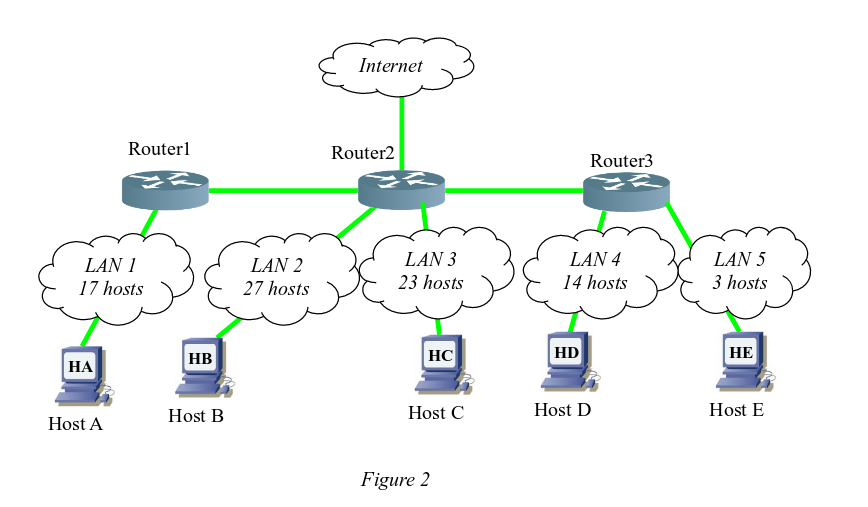
\includegraphics[scale=0.3]{5-network-two}
    \caption{Network topology 2 from Assignment 5.}
    \label{fig:network-two}
\end{figure}

\subsection{}

We need 7 subnets to share the original address space (i.e. 192.168.11.0/24). 

\subsection{}

If we subnet the topology with 7 subnets we will have address allocation as can be seen in the table \ref{tab:2-subnet}. 

\begin{table}[!h]
    \centering
    \begin{tabular}{|c|c|c|c|}
    \hline
    Subnet Name & Addresses Needed & Addresses allocated & Subnet address\\
    \hline
         LAN2 &  28 & 30 & 192.168.11.0/27 \\
         LAN3 &  24 & 30 & 192.168.11.32/27 \\
         LAN1 & 18 & 30 & 192.168.11.64/27 \\
         LAN4 & 15 & 30 & 192.168.11.96/27 \\
         LAN5 & 4 & 6 & 192.168.11.128/29 \\ 
        Router 1-2 & 2 & 2 & 192.168.11.136/30\\
        Router 2-3 & 2 &2 & 192.168.11.140/30 \\
        \hline
    \end{tabular}
    \caption{Address allocations for the subnet topology of exersice 2.}
    \label{tab:2-subnet}
\end{table}




\section{VLSM exersice 3}

\subsection{What is the last valid host on the subnet $172.100.218.0/23$ ? }

The last valid host on the subnet $172.100.218.0/23$ is $172.100.219.254$.

\subsection{What is the first valid host in the subnet that host $192.168.248.69/29$ belongs to?}
The first valid host in the subnet with the host $192.168.248.69/29$ is $192.168.248.65$.
\subsection{What is the last valid host on the subnet $10.0.96.0/20$ ?}

The last valid host on the subnet $10.0.96.0/20$ is $10.0.111.254$.

\subsection{Which subnet does host $192.168.1.98/25$ belong to?}

The host $10.0.96.0/20$ belongs to the subnet $192.168.1.0/25$.

\subsection{What is the last valid host on the subnet $192.168.50.80/28$ ?}

The last valid host on the subnet $192.168.50.80/28$ is $192.168.50.94$. 

\subsection{What is the broadcast address for the IP address $10.0.100.202/26$ ?} 

The broadcast address for the IP address $10.0.100.202/26$ is $10.0.100.255$.

\subsection{Which subnet does host $172.27.117.82$ with sub-net mask $255.255.255.252$ belong to?}

The host $172.27.117.82$ with the subnet mask $255.255.255.252 (/30) $ belongs to the subnet
$172.27.117.80/30$.

\subsection{How many subnets and hosts per subnet can you get from the network $192.168.10.0/27$? You can assume you have a 24-bit network available.}

The number of subnets that we can get is $ 8 (2^3 = 8) $ and the number of hosts that can be connected is $ 30 ( 2^5 = 32-2 = 30) $. The two addresses that are subtracted is the network address (the first address $192.168.10.0 $) and the broadcast address (the last address $ 192.168.10.31$). 

\subsection{What is the last valid host on the $192.168.246.40/29$ subnet?}
The last host on the subnet $192.168.246.40/29$ is $192.168.246.46$.

\subsection{What is the broadcast address of the $192.168.42.192$ network with a subnet mask of 
$255.255.255.192$ ?}

The broadcast address of the network $192.168.42.192$ with the subnet mask of $255.255.255.192 (/26)$ is $192.168.42.255$.

\subsection{How many subnets and host per subnet can you get from the network $172.16.0.0/23$? You 
can assume you have a 16-bit network available.}

The number of subnets that we can get from the network $172.16.0.0/23$ (with a 16-bit available network)  is 64 ($2^7 = 64$). The number of hosts is 510 ($ 2^9 = 512 -2 = 510$). The network and the broadcast addresses are subtracted as we can not assign it to hosts.
 
\subsection{What valid host range is the IP address $192.168.137.219$ with a subnet mask $255.255.255.224$ a part of?}

The IP address $192.168.137.219$ with the subnet mask $255.255.255.224 (/27)$ is in the host range 
$192.168.137.193$ - $192.168.137.222$

\section{OSPF}

\subsection{Reconfiguring the site with routers running OSPF instead of RIP.}

We change all the routing protocols in the routers from RIPv2 to OSPF. To do this we use \textit{vtysh}. We use the command:\\
\begin{itemize}
    \item sudo vytsh 
    \item config t
    \item no router rip
    \item router ospf
    \item network [network address/subnet mask] area [area no.]
\end{itemize}
Here the [network address/subnet mask] is the network address with the subnet mask that the router is directly connected to, and I have used area 0 throughout the site. Then exit into the main quagga command line when we can see \textit{hostname\#} 
and \textit{write}. To save the configuration, and use \textit{filetool.sh} to save it persistently. These changes are done for all the routers, we can see Figure \ref{fig:router3-ospf} for an example.

\begin{figure}[!h]
    \centering
    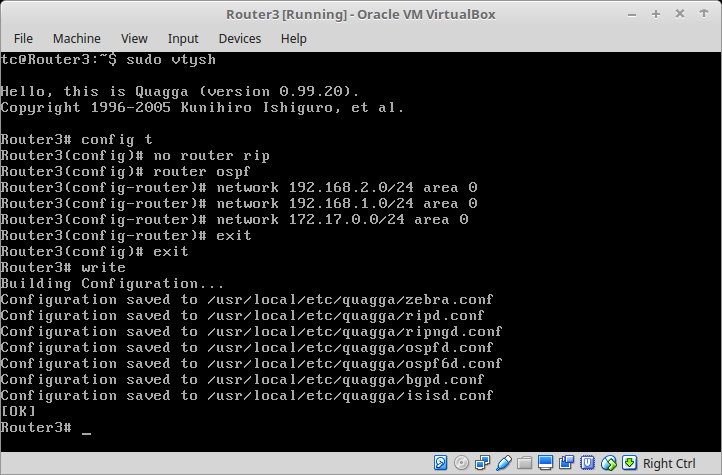
\includegraphics[scale=0.3]{router3-ospf-vtysh}
    \caption{Setting OSPF with \textit{vtysh} at Router3}
    \label{fig:router3-ospf}
\end{figure}


In Figure \ref{fig:GW-routes} we can see the routing table running with OSPF protocol.

\begin{figure}[!h]
    \centering
    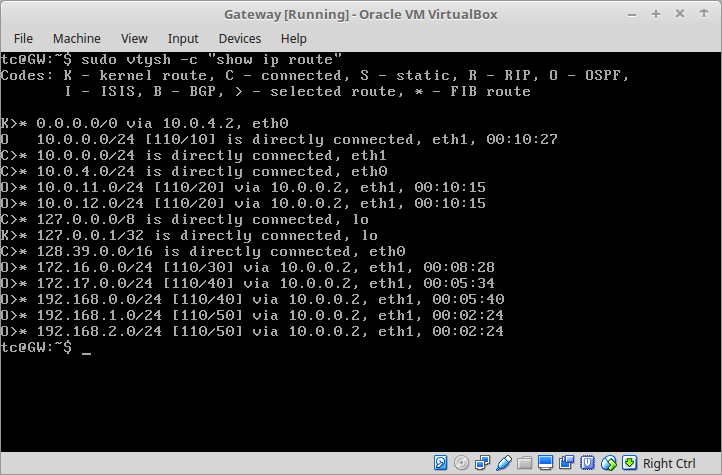
\includegraphics[scale=0.3]{gateway-vytsh-route}
    \caption{Routing table at Gateway}
    \label{fig:GW-routes}
\end{figure}



\subsection{Write a script on H2 that checks for reachability throughout your site, and to the Internet. Use script to document reachability.}

To check the reachability throughout the site, and to the Internet we will use the \textit{ping} command. First we will add all the host names and thier IP addresses to the \textit{/etc/hosts} file at Server2. As Server2 is the nameserver for all the hosts and nodes in the network. 
We add the hostname and its corresponding IP address with the \textit{echo} command at the \textit{bootlocal.sh} file at Server 2. Then save it persistently with \textit{filetool.sh}. The \textit{bootlocal.sh} file with all the hostname and thier IP addresses can be seen in Figure \ref{fig:server2-lst}. 

\begin{figure}[!h]
    \centering
    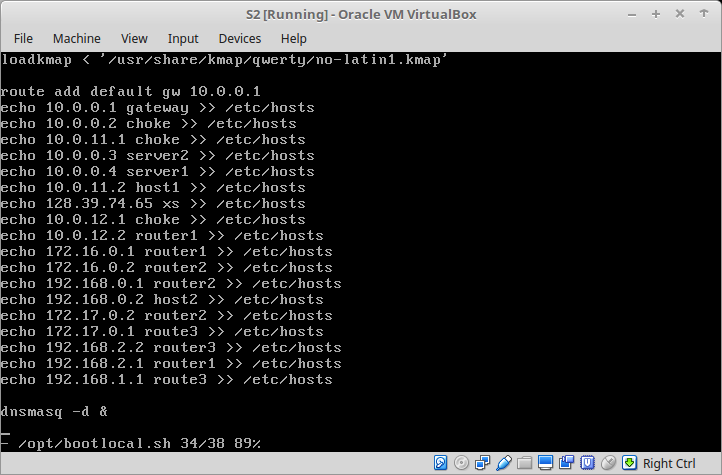
\includegraphics[scale=0.3]{server2-host-list}
    \caption{Server 2 \textit{bootlocal.sh} file, host list}
    \label{fig:server2-lst}
\end{figure}

Then at Host 2 we make a file with all the hosts and the internet domain name. In our script we will read through this file with the \textit{cat} command and \textit{pipe} it to a while loop to execute the \textit{ping} command for each hostname. This can be seen in Figure \ref{fig:host2-file}. 
\begin{figure}[!h]
    \centering
    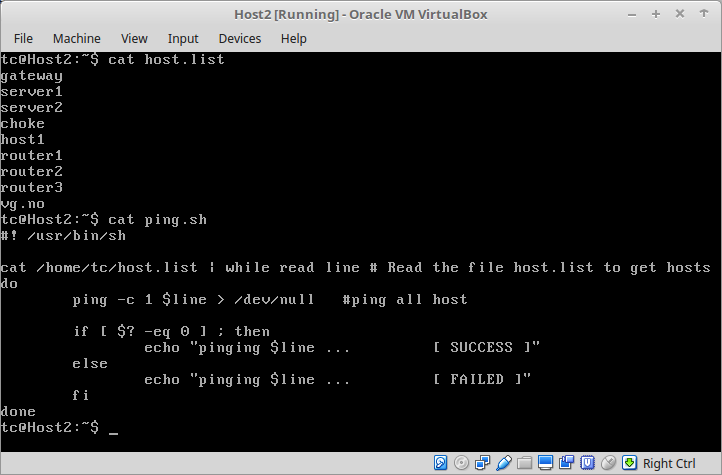
\includegraphics[scale=0.4]{host2-ping-file}
    \caption{The \textit{host list} and the script at Host 2}
    \label{fig:host2-file}
\end{figure}

Executing this command we got a successful result as seen in Figure \ref{fig:host2-pinging}.

\begin{figure}[!h]
    \centering
    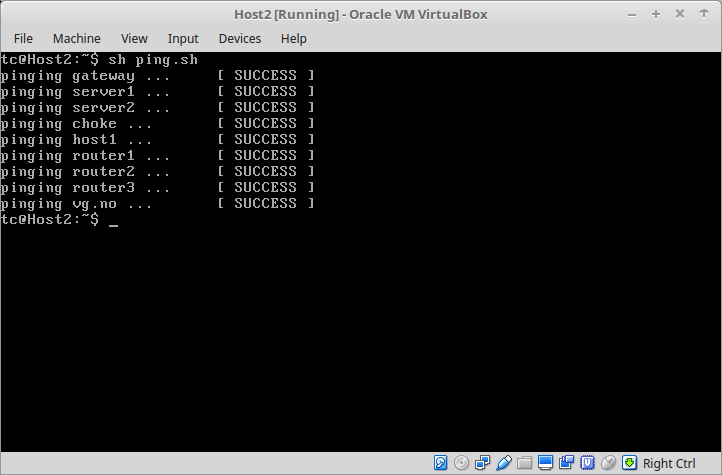
\includegraphics[scale=0.3]{host2-pinging}
    \caption{Results for executing the script at Host 2}
    \label{fig:host2-pinging}
\end{figure}

\section{Planning the subnetting of the site}

Here the site seen in Figure \ref{fig:site-top} will be subnet-ed using VLSM. We do not implement this configuration in the site iteself, but just plan and illustrate it.


\subsection{Using VLSM to subnet the site.} 

To subnet the site with VLSM, we need to add one to the hosts required in the assignment text as we need to assign an IP address to the router as well, two in case of the DMZ subnet. We need to assign the largest block to the "D1cable"-subnet (where Host 1 is located) as it needs the most number of hosts (i.e. 35+ 1 router) which is 36. So we assign it a block of 64 addresses, which can have 62 hosts and has a network and broadcast address. Similarly we assign hosts to all the subnets and the point-to-point links, which is also a subnet. The final result can be seen in Table \ref{tab:vlsm-site}. The poin-to-point links with the routers are named as subnet "Rx-Ry", where x and y are router numbers.

\begin{table}[!h]
    \centering
    \begin{tabular}{|c|c|c|c|}
    \hline
         Subnet name & Required Hosts & Available hosts & Network addresses/Subnet Mask    \\
         \hline
         D1cable & 36 & 62 & 10.0.0.0/26 \\
         Wireless\_access\_cable & 13 & 14 & 10.0.0.64/28 \\
         DMZ & 4 & 6 & 10.0.0.80/29 \\ 
         D2cable & 4 & 6 & 10.0.0.88/29\\
         R2-R3 & 2 & 2 & 10.0.0.96/30 \\
         R1-R2 & 2 & 2 & 10.0.0.100/30 \\
         R1-R3 & 2 & 2 & 10.0.0.104/30 \\
         R1-Chk & 2 & 2 & 10.0.0.108/30\\
         \hline
    \end{tabular}
    \caption{VLSM for the site seen in Figure\ref{fig:site-top}}
    \label{tab:vlsm-site}
\end{table}

\begin{figure}[h]
    \centering
    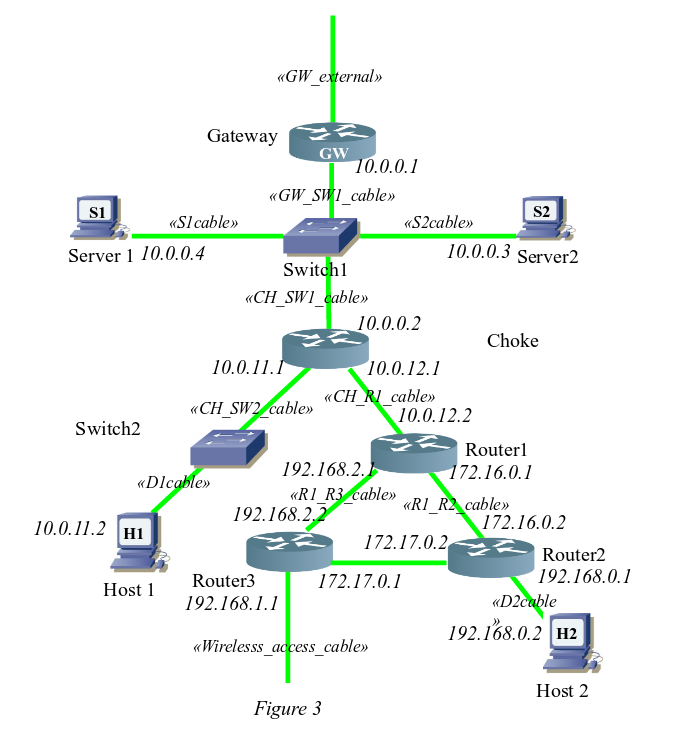
\includegraphics[scale=0.3]{net-top-site}
    \caption{The network topology of our site}
    \label{fig:site-top}
\end{figure}

\part{Discussion}

Running the ping command on Host 2 after initially after all the nodes and hosts have just been booted up it takes Host 2 some time to \textit{ping} the Internet. The \textit{ping} command fails to ping at the first try but after a few seconds it pings, successfully. 

\begin{thebibliography}{9}
\bibitem{textbook}
  James F.Kurose, Keith W. Ross,
  \emph{Computer Networking},
  PEARSON, 
  6$^{th}$ edition,
  2012.
\end{thebibliography}

\end{document}
